\chapter{State of the art}
\label{c:sota}

Intrusion detection is, as defined in \cite{Liao2013}, “the process of monitoring the events occurring in a computer system or network, and analysing them for signs of intrusions”. It can be deployed directly on the network node (host-based), where it monitors the activity for hosts containing sensitive information, or it can be deployed on the network (network-based), where it monitors traffic using sensors. Recent literature classifies the system’s detection approach as being either signature-, anomaly-, or specification-based \citep{Lokman2019}.

\section{Detection approaches}
\label{sec:ids_detection_approaches}

A signature-based \gls{ids} raises an alert when it finds a pattern in the network that corresponds to a signature in the system database. Its advantage comes from its simplicity, as it only requires a database of known attacks to compare network traffic to. However, this reliance on the attack signature database means that it will not recognise new attacks that are not stored there, meaning that regular updates are required.\par
The specification-based approach attempts to detect deviations from a protocol specification (well-defined rules that describe component behaviour). It is, again, a simple solution that requires only a set of rules that trigger an alert when not followed. Nonetheless, manually setting specifications is an error-prone and time-consuming task and must be adapted for different domains.\par
In the case of an anomaly-based \gls{ids}, an alert is raised when the network state deviates from what it considers to be normal behaviour. Here, the challenge relies upon defining what is considered normal behaviour, as a poorly defined model can generate alerts on what would otherwise be considered normal packets. A high rate of false positives could cause the driver to ignore the alerts completely. Techniques for defining what constitutes normal behaviour include machine learning, packet frequency and statistical-based analysis, as well as a hybrid approach.\par
In the traditional desktop environment, a hybrid approach is a combination of several \gls{ids} techniques, such as network- and host-based \gls{ids}. Here, the host-based \gls{ids} aggregates information into a standard format, which is then transmitted to the network-based \gls{ids}, where it is aggregated and processed. In the case of anomaly detection in \gls{can}, a hybrid-based approach consists of the combination of more than one detection method, considering various packet features, e.g., ID field, payload, timing interval and frequency \cite{Lokman2019}.

\section{IDS evasion techniques}

Intrusion detection systems are commonly used in many networks, and attackers have adapted in order to avoid being detected. Evasion techniques mostly make the use of fragmentation, flooding, obfuscation and encryption.\par
Fragmentation is the process of dividing a packet into smaller packets, which are then reassembled when received. To analyse these fragmented packets, an \gls{ids} is required to re-assemble them. Attackers then take advantage of fragmentation overlap, overwrite and timeouts to escape detection. Flooding occurs when an attacker overwhelms the detector with a massive stream of packets, which causes it to fail. Obfuscation works by making a message difficult to understand, typically by changing the code while maintaining its functionality. This reduction in the code readability makes both static analysis and reverse engineering much more difficult. An \gls{ids} using a signature database will also see a decrease in its ability to detect attacks. Although encryption offers many security benefits, attackers can also leverage it to their advantage. Attacks on encrypted protocols, for example, cannot be detected by an \gls{ids} that relies on a signature database, as it cannot interpret the packets contents \citep{Khraisat2019}.

\section{Intrusion detection in the Controller Area Network}
\label{sec:can_ids}

Although \glspl{ids} are commonplace in traditional IP networks, they are still being developed for use in vehicles, more specifically in the \gls{can} bus. Therefore, there still is no single best approach, but multiple different attempts to build a reliable \gls{ids}.

\subsection{Based on packet frequency}

\cite{taylor2015frequency} proposed a frequency-bases analysis of network traffic flow in order to detect anomalies. Through the use of a \gls{ocsvm}, they found that they were able to identify when packets were artificially inserted or removed by the mean-time interval between packets of the same ID. Another frequency-based detection method was proposed by \cite{song2016intrusion}, in which they recorded no false positives during the packet injection tests.\par
An \gls{ids} that is based on the offset ratio and time interval between request and response was proposed by \cite{lee2017otids}. The system periodically sends remote frame requests and analyses the response time, and attacks were successfully identified because of the abnormalities in the instant reply ratio, lost reply ratio, correlation coefficient between offsets and time intervals, and average response time.\par
A clock-based \gls{ids} was developed by \cite{cho2016fingerprinting}, where it identified \glspl{ecu} based on the intervals of periodic messages. This baseline then allowed for the detection of abnormal behaviour in the network, with a reported false positive rate of 0.055\%. Unlike most \glspl{ids}, it also facilitated the identification of the misbehaving \gls{ecu}.

\subsection{Based on network entropy}

An entropy-based anomaly detection mechanism was proposed in \cite{muter2011entropy}. Here, the developed \gls{ids} analysed variation in the network entropy (\textit{i.e.}, how much coincidence a given dataset contains) to detect anomalies. Through increased message frequency, message flooding, and simulation of unrelated events, they concluded that "deviations from the normal behavior of in-vehicle networks can successfully be identified by an information-theoretic detection approach". Another entropy-based system was proposed by \cite{marchetti2016evaluation}, in which they claimed that this represents a "viable approach for identifying CAN bus anomalies caused by the activity of attackers that [are] injecting messages over the CAN bus". However, limitations include only being able to detect attacks where packets are inserted at a high rate.

\subsection{Based on network data probability}

\cite{kang2016intrusion} used probability-based feature vectors extracted from the network packets to train a \acrlong{dnn}. The training was performed offline, while the detection was done against incoming packets in the network. They achieved a 99\% detection racio against a \gls{tpms} spoofing attack. Another deep learning model was presented in \cite{Taylor2016}, in which the authors developed an \gls{lstm} that attempts to predict the next data word originating from each sender on the bus, flagging anomalies. However, it worked only for a single CAN ID and did not support online learning.\par
In \cite{narayanan2016obd_securealert}, the authors proposed the utilisation of a \gls{hmm} to model what is considered normal vehicle function. The \gls{ids} works by signalling low probability changes of state (like a sudden jump from 25 kph to 160 kph) as an anomaly. The system was able to detect the introduction of anomalous RPM data, and they state that advantages of this approach include the fact that it can be applied in a plug-and-play fashion to both new and older vehicles.

\subsection{Hybrid}

\cite{weber2018embedded} presented a hybrid anomaly detection system that combines both specification-based detection and machine learning, drawing from the advantages of both. In a first stage, static checks are made, and then the machine learning part applied learning checks for temporal analysis of the \gls{can} packets.\par
A \gls{htm} model was developed by \cite{wang2018distributed}. This is a memory-based model that is capable of online learning, meaning that it can continuously learn with new \gls{can} data. Results from packet insertion and modification attacks show that it outperforms existing \gls{can} \glspl{ids} that used \gls{rnn} and \gls{hmm} models.

\subsection{Based on protocol specifications}

The authors of \cite{larson2008approach} investigated the use of a specification-based \gls{ids} with security rules derived from the e \gls{can} v2.0 and CANopen draft standard 3.01 communication protocol and object directory sections. These enforce the correct functioning of the protocol according to specification, signalling deviation from the rules as anomalous traffic. They tested six types of attacks (spoof, replay, read, modify, flood, and drop), concluding that most attacks can be readily detected and that "both protective and detective measures will be required in future in-vehicle networks".

\subsection{Based on attack signatures}

\section{Challenges for automotive}

There are, however, several challenges that must be overcome to successfully implement an \gls{ids} in a \gls{can} bus. First, most \glspl{ecu} have very limited resources, meaning low memory capacity, computational power, and data transmission rate. Another consideration is the time-sensitive nature of the packets being transmitted \citep{hoppe2009applying}. Proper vehicle function must be maintained, which means that \gls{can} packets must be managed in real-time. Otherwise, the safety of the driver might be at risk, as there would be an additional delay in information processing. Typical \gls{ids} solutions were developed for conventional Internet Protocol (IP) networks. As this is environment is very different from the in-vehicle one, adopting existing solutions is not possible. The nature of the vehicle environment is also a constantly moving one, and at various speeds. This means that an \gls{ids} must have a certain degree of autonomy, as establishing a connection to an outside party may not always be possible. Lastly, it must be an efficient solution, both in terms of cost, for it to be implemented in mass-production, and its physical aspects, i.e., not requiring massive amounts of rewiring, as it may be infeasible for manufacturers \citep{Lokman2019}.\par
In a traditional IT setting, a system administrator is usually in charge of maintaining the system functioning properly and up to date, and is also the one notified in case of an alert. In the automotive domain, however, the \gls{ids} cannot be maintained by a qualified administrator, and a typical user cannot be expected to be an IT expert. This means that tasks like maintenance and alert handling can be delegated to him in a limited way. This might motivate the design of the system to be as autonomous as possible, but the high safety requirements of automotive systems make this a challenging task. The authors of \citep{hoppe2009applying} state that "in general, automotive systems shall never take safety relevant decisions autonomously but may only support the driver in his reaction (final decisions regarding control or safety of the vehicle are only to be made by the driver)". Because of this, special care must be taken when deciding upon the way of communicating an alert to the driver. This communication must be done in a modern way, taking advantage of the car's multimedia system, and must not cause panic. If a driver reaction is required, it is advantageous to provide suggestions, and the need to disrupt the driver must be kept to a minimum. They suggested a gradual approach to this communication, depending on the severity of the incident, which can be seen in Figure \ref{fig:ids_communication}. From left to right, as the severity of the incident increases, the amount of time it takes to grab the attention of the driver reduces. A visual-only message would be read when the driver decides to look at the display, but a haptic intervention would cause immediate alert. However, the amount of information that can be communicated is reduced, as a visual or acoustic message would reveal more about the incident that a haptic intervention.

\begin{figure}
    \centering
    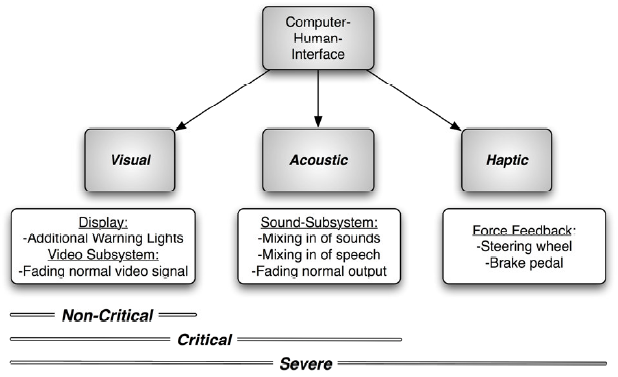
\includegraphics[width = \textwidth]{img/parts/introduction/IDS Communication.png}
    \caption{Stages for alert communication \citep{hoppe2009applying}}
    \label{fig:ids_communication}
\end{figure}

\section{Incident response}

Unlike in other settings where an \gls{ids} might be used, like in desktop IT, one can no expect that the typical vehicle user is an IT expert. Therefore, maintenance and alert handling can be delegated to the driver in only a very limited way.\par
The lack of a knowledgeable user might motivate building a system that is as self-contained as possible. This would include being able to respond do intrusions. However, such an intrusion response mechanism is challenging to build given the high safety requirements of the automotive domain. Therefore, it is important to consider how the system should respond in case it detects an attack. \cite{hoppe2009applying} identified four aspects that should be taken into consideration when designing a way to communicate an alert to the driver: the use of a modern way of communicating, transmission of a sense of peace of mind, avoiding repetition, and support of the driver's decision making. They then propose a three-stage model, which can be seen of Figure \ref{fig:ids_adaptive_dynamic_reaction} for alert communication to the driver depending on the severity of the intrusion. The three stages are visual, containing elements like the dashboard or central screen, acoustic, through the vehicle's sound system, and haptic, through force feedback in the break pedal or steering wheel.

\begin{figure}
    \centering
    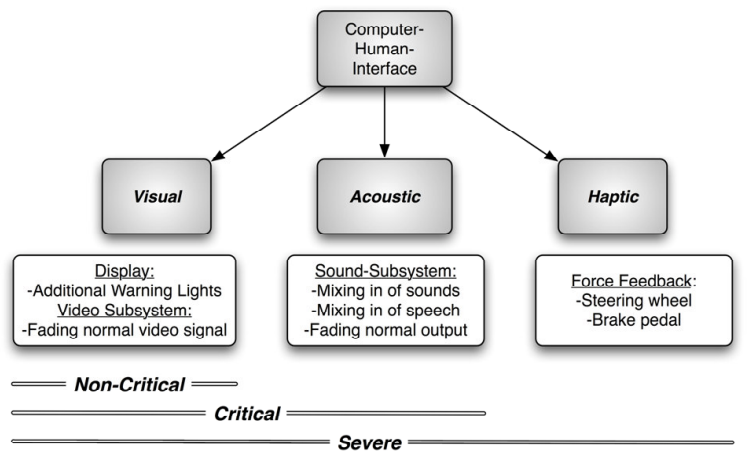
\includegraphics[width = \textwidth]{img/parts/app/Adaptive IDS Alarm System.png}
    \caption{Three stages model for IDS alert communication \citep{hoppe2009applying}}
    \label{fig:ids_adaptive_dynamic_reaction}
\end{figure}

Increasing severity is implicated by going from visual to acoustic and then to haptic. A visual-only message is used for non-critical alarms as the driver may not immediately look at the visual indication. Combining visual with acoustic signals indicates a critical alarm, as the driver would be immediately alerted. Haptic signals, like steering wheel vibration, is reserved for only severe alarms as it might frighten the driver. However, communication ability increases by going from haptic to acoustic and the to visual. Haptic signals are only able to indicate that something is wrong, without further information. Audible signals are able to provide more context, with visual messages informing the driver about what is the problem.\par
The severity of the alarm, however, is not the only factor to determine what stage should be used. Environmental context gathered from the vehicle's multiple sensors may aid in this decision. If the light sensors, for example, detect a high level of brightness, the system may opt for audiovisual indication in a non-critical situation, as a visual-only warning would be difficult for the driver to notice.